\section{Technique}
%
To add path merging to SPF, we first pre-compute static summaries of arbitrary code regions with more than one execution
path and we also pre-compute method summaries.\\
%
To bound the set of code regions we analyze, we start by specifying a method $M$ in a configuration file.
%
Next, we construct a set containing only the class $C$ that contains $M$.
%
We then get another set of classes, $C'$,
such that every class in $C'$ has at least one method that was called by a method in a class in $C$.
%
This step which goes from $C$ to $C'$ discovers all the classes at a call depth of 1 from $C$.
%
We continue this method discovery process up to a call depth of 2.\\
%
While we can increase the call depth in our method discovery process, we found that summarizing
arbitrary code regions with more than 2 calls deep, did not lead to practically useful region summaries.\\
%
After obtaining a list of methods, we computed static summaries of regions in these methods and method summaries as
explained in Section \ref{sec:static-analysis}.
%
After computing static region and method summaries, we process them as a sequence of transformations described in the next section~\ref{sec:instantiationTransformations} and summarized
in Figure~\ref{fig:overview}.
%
\begin{figure}[]
    \caption{Overview of transformations on Ranger IR to create and instantiate multi-path region summaries with higher-order regions}
    \label{fig:overview}
    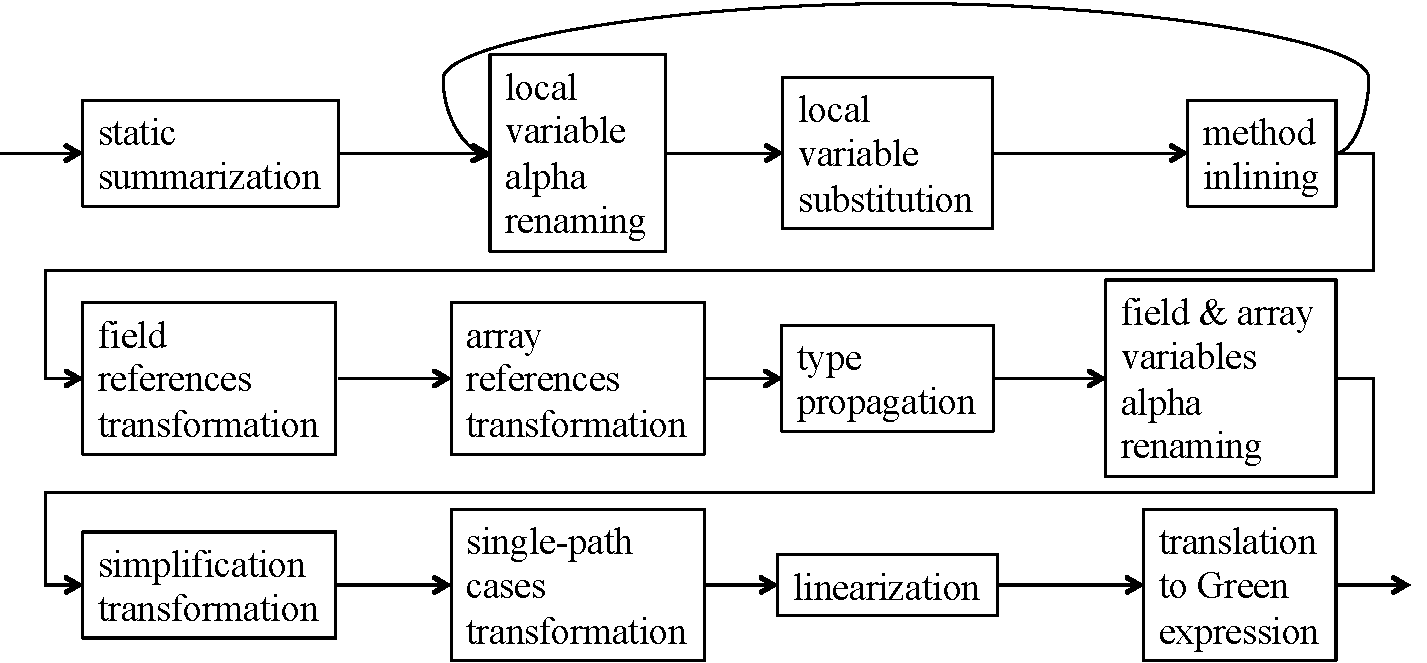
\includegraphics[width=\textwidth]{figures/overview.pdf}
\end{figure}
%
%
%\subsection{WALA-based analysis for veritesting}
%%
%Veritesting requires static construction of
%predicates of a multi-path region which represent changes to the path expression of the dynamic
%symbolic executor.
%%
%It also requires construction of a control-flow graph of method bodies
%from Java bytecode and finding exit points of the region, which in turn
%requires creation of a control-flow graph of the region.
%%
%Implementing veritesting is made simpler by using a static single
%assignment~(SSA)~\cite{ssa} representation of the multi-path region.
%%
%Using an SSA form allows us to use the $\phi$-expressions created by the
%SSA form and translate them into points at the end of the veritesting
%region where updates to system state along different paths in the region
%can be merged.
%%
%\mike{MWW: Vaibhav please update to describe WALA}
%WALA~\cite{} is a static analysis framework for Java programs that
%has both these features, with
%ExceptionalUnitGraph~\cite{exceptionalunitgraph} and the Shimple
%IR~\cite{shimple}.
%%
%For simple regions with only one exit point, like the one presented in Listing~\ref{lst:v_ex}, we
%were able to use Soot to automate static construction of the predicate representing
%an update to the expression.
%%
%For doing this, we used nodes with more than one successor as the
%starting point, found the immediate post-dominator of the starting
%point, and traversed the control-flow graph on all sides of such branches.
%%
%During such a traversal, we constructed predicates representing the
%multi-path region, similar to the ones presented in
%Listing~\ref{lst:v_ex_smt2}.
%%
%As explained in Section~\ref{sec:exit_points}, including virtual
%function invocations in the construction of our predicates amplifies the
%benefits of veritesting even further.
%%
%We plan to automate this inclusion in the future using Soot.
%%
%Providing SPF with updates to be made to its symbolic store also
%requires Soot to maintain stack location information for variables.
%%
%We plan to automate SPF\rq s symbolic store updates using Soot in the
%future.
%%
%

\subsection{Statement Recovery}
\label{sec:static-analysis}
%Java Ranger has its own AST that captures the statement of regions.
%%
%The choice of having a separate AST for Java Ranger, enables the integration of Java Ranger with any static analysis framework by implementing the transformation that transforms the CFG of a given IR into the corresponding Java Ranger AST representation. 
%%
%We call this interface \textit{Statement Recovery} transformation. \\
%%
%In this transformation we visit nodes in topological order by walking normal edges of a branching points until a \textit{minimum convergent node} is encountered. We define a minimum convergent node as the last immediate successor of blocks following a branching node.
%%
%Note that exceptional edges are ignored during this transformation, however exceptional behavior is later identified and handled through the single path cases.
%%
%We discuss more about this in section~\ref{sec:instantiationTransformations}.
%%
%There are two other things that this transformation takes care of: recovering of complex if-then-else and construction of Gated Single Assignment (GSA).
%%
%Recovering of complex conditions in an if-statement restores its form in the source code. 
%% 
%This is done by identifying \textit{immediate self-contained subgraphs}, that is, subgraphs where the initial node is immediately pre-dominated by the initial node and for the static region and whose successor nodes (up to the region terminus) are dominated (not necessarily immediately) by the initial node.
%%
%
%Construction of Gated Single Assignment (GSA) on the other hand is done by keeping track of the current "conditional path" during translation. More precisely this is done by keeping a stack of  {\tt(Expression x enum \{Then, Else\})} pairs. 
%%
%In addition to that, for each edge between blocks in the block structure, the associated "conditional path" is recorded.  
%%
%So the type of this map (the blockConditionMap) is: {\tt(ISSABasicBlock x ISSABasicBlock) --> List of (Expression x enum \{Then, Else\})}.
%%
%Finally creation of the condition of GSA is done during translating a phi-instruction its immediate predecessor blocks are retrieved then we look up  the edges in the blockConditionMap.  From here, and using condition stack leading to that branch, an if/then/else statement is constructed.

The regions of interest for our technique are bounded by the branch and meet of a given acyclic subgraph.  The intuition is that path explosion during execution of loops is driven by conditional logic within the loop, rather than the loop itself.
Starting from an SSA form, the first transformation recovers a tree-shaped AST for the subgraphs of interest.  While this step is not strictly necessary, it substantially simplifies subsequent transformations.  

The algorithms are similar to those used for those used for decompilation~\cite{Yakdan15@decompilation} but with slightly different goals: 
\begin{itemize}
    \item The algorithm must be {\em accurate} but need not be {\em complete}.  That is, obfuscated regions of code need not be translated into a tree form.
    \item The algorithm must be {\em lightweight} in order to be efficiently performed during analysis.  Thus, algorithms that use global fixpoint computations are 
        too expensive to be used for our purposes.
\end{itemize}

Starting from an initial SSA node, the algorithm first finds the immediate post-dominator of all {\em normal} control paths, that is, paths that do not end in an exception or return instruction.  It then looks for nested self-contained subgraphs.  If for any graph, the post-dominator is also a predecessor of the node, we consider it a loop and discard the region.  

The algorithm systematically attempts to build regions for every branch instruction, even if the branch is already contained within another region.  The reason is that it may not be possible to instantiate the larger region depending on whether summaries can be found for {\em dynamically-dispatched} functions, and whether references are {\em uniquely determinable} for region outputs.

\iffalse
\begin{verbatim}

stmt ::= stmt ; 
   

\end{verbatim}

\vaibhav{assigned to Mike}
\mike{MWW: - we should provide an AST of the constraint language}
\fi 

\subsection{Region Definition}

Once the statement of a Ranger region has been recovered, its corresponding environment is populated. This includes identifying region boundary and creating input, output, type and stack slot tables for the region.

The region boundary is used to identify boundaries of the region as opposed to exploring the whole IR. This is used later to constrain the computation and population of different environment tables. For example, input table is populated with first use in the region boundary that map to a given stack slot. The output table is populated with the last def, if a converging statement exits. Type table is populated for all variables that lay within the boundaries of the region, this is initially done by inquiring the static analysis framework, WALA~\cite{Wala} but later undergoes some changes during type propagation transformation~\ref{sec:instantiationTransformations}. 

The stack slot table on the other hand, does not use region boundary for its population. The reason for this is that, the static analysis framework we use, WALA, sometime does not provide information about the stack slots of intermediate variables. This is particularly problematic in our case because the def of a phi is both an intermediate variable, and so we do not know its stack slot, yet it is also an output of the region for which we want to populate its symbolic representation onto the stack slot. Therefore, our stack slot table uses stack slot inference by propagating the stack slots of vars used in a phi onto the def of the phi. This requires visiting all variables and phi statements of the IR to maximize the inference of the stack slot, this is repeatedly done until a fix point is reached.


\subsection{Instantiation-time Transformations}
\label{sec:instantiationTransformations}

\textbf{Renaming Transformation}: In Alpha renaming transformation, all Ranger IR variables are renamed to ensure their uniqueness before further processing takes place. 
%
This is particularly important not only to ensure uniqueness of variables among different regions, but also to ensure
uniqueness of variable names of the \textit{same} region which might be instantiated multiple times on the same path,
i.e., a region inside a loop will be instantiated multiple times.\\
%
\textbf{Local Variable Substitution Transformation}: During this transformation we eagerly bring in all dynamically
known constant values, symbolic values and references from stack slots into the region for further processing. \\
%
\textbf{Higher-order Regions Transformation}: This transformation is initiated when a method invocation is encountered
during local variable substitution.
%
At this point, we perform three steps.
%
(1) the region that corresponds to the called method is retrieved and alpha renaming of
Ranger IR variables corresponding to local variables is applied on it.
%
(2) Ranger IR expressions that correspond to the actual parameters are evaluated and used to substitute the formal
parameters by repeatedly applying local variable substitution transformation over the method region.
%
(3) When no more higher-order regions can be inlined, the resulting substituted method region is inlined into
the outer region.\\
%
If the method region has a single return value, then the original method invocation is replaced with an assignment to
the returned expression.
%
%Otherwise, inlining of the method region takes place.
%
We dont currently support instantiation of method regions with multiple return statements, support for which requires
another transformation that we talk about in Section~\ref{sec:future}.
\\
\textbf{Field References SSA form}: The field references transformation translates reads and writes of fields
in Java bytecode into corresponding Ranger IR statements.
%
In order to translate all field accesses to SSA form, this transformation creates a summary of the semantics
represented by the field accesses in the region.
%
This transformation constructs a new field access variable for every field assignment on every path within the region.
%
This new field access variable construction makes use of two monotonically increasing subscripts.
%
It uses a path subscript to distinguish between assignments to the same field on the same execution path.
%
It uses a global subscript to distinguish between assignments to the same field across execution paths.
%
At the merge point of the region, field assignments done on the same field are merged using
Gated Single Assignment (GSA)~\cite{Ottenstein1990}.
%
Each merged field access variable has its own path and global subscripts and represents the output of the region into
its field.
%
The path subscript helps us resolve read-after-write operations on the same execution path and find the latest write
into a field on an execution path.
%
The global subscript helps us distinguish between field accesses across multiple execution paths. \\
\textbf{Array References SSA form}: The array references transformation translates reads and writes of arrays in
Java bytecode into corresponding Ranger IR statements.
%
In order to translate all array accesses to SSA form, this transformation creates an execution path-specific copy of
every array when it is first accessed within a region.
%
Reads and writes of arrays are then done on a path-specific copy of the array.
%
All array copies are merged at the merge point of multi-path regions.
%
The merged array copy represents array outputs of the region.\\
\textbf{Type Propagation}: Ranger IR needs to have type information for its variables so that it can construct
corresponding correctly-typed Green variables during the final transformation of the region summary to a Green formula.
%
Having accurate type information is also important for looking up the correct higher-order method summary.
%
As part of region instantiation, Java Ranger infers types of Ranger IR variables in the region summary by
using JPF's runtime environment.
%
Types of local variables are inferred during the local variable substitution transformation and types of field reference
and array reference variables are inferred during their respective transformations.
%
Using these inferred types, the type propagation transformation propagates type information across assignment
statements, binary operations, and variables at leaf nodes of $\gamma$ functions.\\
%
\textbf{Simplification of Ranger IR}: The Ranger IR constructed by earlier transformations computes exact semantics
of all possible behaviors in the region.
%
Representation of such semantics as a formula can often lead to unnecessarily large formulas, which has the potential to
reduce the benefits seen from path merging~\cite{angr}.
%
For example, if an entry in an array is never written to inside a region, the array reference transformation can still have an
array output for that entry that writes a new symbolic variable into it.
%
The region summary would then need to have an additional constraint that makes the new symbolic variable equal the
original value in that array entry.
%
Such conjuncts in the region summary can be easily eliminated with constant propagation, copy propagation, and constant
folding~\cite{dragon-book}.
%
Ranger IR also has statement and expression classes that use a predicate for choosing between two statements (similar to
an {\tt if} statement in Java) and two sub-expressions (similar to the C ternary operator) respectively.
%
When both choices are syntactically equal, the predicated statement and expression objects can be substituted with the
statement or expression on one of their two choices.
%
Such statements and expressions were simplified away to use one of their two choices.
%
Ranger IR performs these two simplifications on such predicated statements and expressions along with constant folding,
constant propagation, and copy propagation.\\
\textbf{Single Path Cases}: This transformation collects path predicates inside a region that lead to
\textit{non-nominal} exit point.
%
This is an alternative approach to that was presented in \cite{veritesting}.
%
In our work we define non-nominal exit point to be points inside the region that either define exceptional behavior or
involve behavior that we cannot summarize, i.e, object creation and throw instructions.
%
The intuition here is that, we want to maximize regions that Java Ranger can summarize, even if the summarization is
only partial.
%
We use this pass of transformation to identify such points, collect their path predicates and prune them away from the
Ranger IR statement.
%
The outcome of this process, is a more simplified and concise statement that represent the nominal behavior of the Ranger region.
%
The collected predicate is later used to guide the symbolic execution to explore non-nominal paths, which Java Ranger
had not summarized.  \\
%
\textbf{Linearization}:
Ranger IR contains translation of branches in the Java bytecode to if-then-else statements defined in the Ranger IR.
%
But the if-then-else statement structure needs to be kept only as long as we have more GSA expressions to be
introduced in the Ranger IR.
%
Once all GSA expressions have been computed, the Ranger IR need not have if-then-else statements anymore.
%
The $\gamma$ functions introduced by GSA are a functional representation of branching, which lets us
capture the semantics of everything happening on both sides of the branch.
%
Since the linearization transformation is done after every field and array entry has been unaliased and converted to
GSA, dropping if-then-else statements from the Ranger IR representation of the region summary reduces redundancy in its
semantics and converts it into a stream of GSA and SSA statements.\\
\textbf{Translation to Green}:
%
At this point Ranger region contains only compositional statements as well as assignment statements that might contain GSA expressions in them.
%
This transformation starts off by translating Ranger variables to Green variables of the right type using the region type table.
%
Then Ranger statements are translated. More precisely, compositional statements are translated into conjunction, assignment statements are translated into Green equality expressions.
%
For assignment statements that have GSA expressions, these are translated into two disjunctive formulas that describes the assignment if the GSA condition or its negation were satisfied. 

\subsection{Checking Correctness Of Region Summaries}
The Ranger IR computed as a result of performing the transformations described in Figure~\ref{fig:overview} should
correctly represent the semantics of the summarized region.
%
If it does not, then using the instantiated region summary can cause symbolic exploration to explore the wrong behavior
of the subject program.
%
We checked the correctness of our instantiated region summaries by using equivalence-checking as defined by Ramos et al.~\cite{ramos}.
%
We designed a test harness that first executes the subject program with a set of symbolic inputs using SPF and
capture the outputs of the subject program.
%
Next, the test harness executes the same subject program with the same set of symbolic inputs using Java Ranger and
capture the outputs of the subject program once again.
%
Finally, the test harness compares outputs returned by symbolic execution with SPF and Java Ranger.
%
If the outputs do not match, then a region summary used by Java Ranger did not contain all the semantics
of the region it summarized.
%
We symbolically execute all execution paths through this test harness.
%
If no mismatch is found between outputs on any execution path, we conclude that all region summaries used by Java Ranger
must correctly represent the semantics of the regions they summarized.
%
We performed correctness-checking on all results reported in this paper.
